\chapter{Requisiti}

\section{Use Case Diagram}
Per definire i requisiti funzionali del sistema in ottica Object-Oriented, si è proceduto all'identificazione degli attori principali e dei relativi casi d'uso. 

Il sistema prevede le seguenti figure:
\begin{itemize}
    \item \textbf{Cliente:} Utente finale che interagisce col sistema per consultare il catalogo e prenotare le esperienze.
    \item \textbf{Game Master:} Personale di filiale deputato al controllo operativo delle stanze e delle sessioni.
    \item \textbf{Admin:} Amministratore di sistema incaricato di definire il catalogo e le logiche commerciali.
\end{itemize}

La Figura \ref{fig:usecase} illustra il diagramma globale dei casi d'uso, evidenziando i confini del sistema (Boundary) e le relazioni di inclusione ed estensione. Si noti come le operazioni critiche (prenotazioni e gestione interna) richiedano obbligatoriamente l'autenticazione tramite la relazione \texttt{<<include>>}, e come la gestione della lista d'attesa rappresenti una pura estensione (\texttt{<<extend>>}) del normale flusso di prenotazione.

\begin{figure}[H]
    \centering
    % Assicurati di aver esportato il png da PlantUML dentro la cartella images
    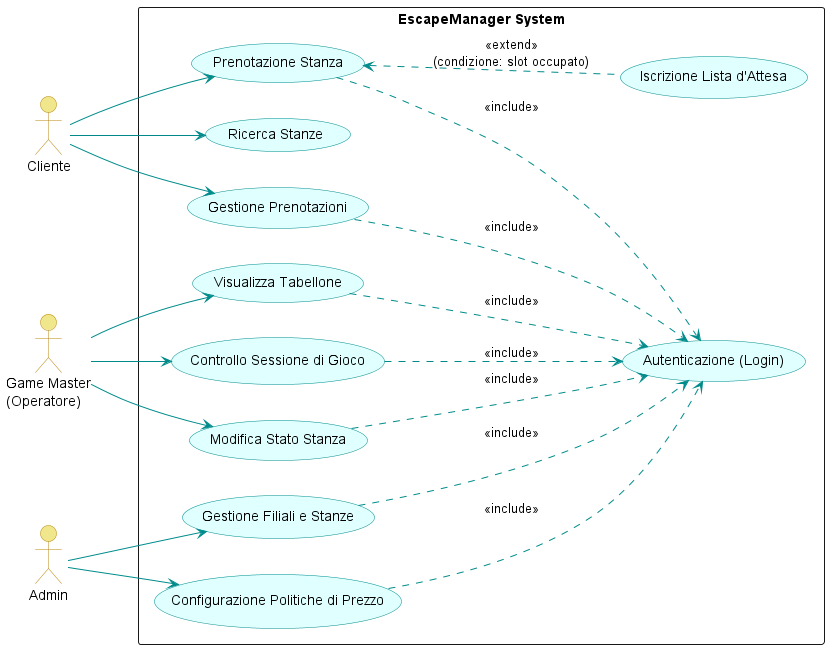
\includegraphics[width=0.85\textwidth]{images/usecase_diagram.png}
    \caption{Diagramma dei Casi d'Uso (Use Case Diagram) di EscapeManager}
    \label{fig:usecase}
\end{figure}

\section{Use Case Templates}
A corredo del diagramma, vengono definiti i template testuali per i casi d'uso primari. La formalizzazione di questi scenari descrive nel dettaglio il Flusso Base (Basic Flow) e i Flussi Alternativi (Alternative Flows), i quali costituiranno successivamente la base per la stesura dei test funzionali e di accettazione.

\subsection{UC1: Prenotazione Stanza}
Questo caso d'uso descrive il processo attraverso il quale un Cliente prenota una sessione di gioco in una specifica Escape Room, scegliendo data, ora e numero di partecipanti. Il sistema si occupa di verificare la disponibilità e calcolare la tariffa applicabile.

\begin{table}[H]
    \centering
    \renewcommand{\arraystretch}{1.3} % Aumenta lo spazio tra le righe
    \begin{tabularx}{\textwidth}{|l|X|}
        \hline
        \textbf{ID Caso d'Uso} & \textbf{UC1} \\
        \hline
        \textbf{Nome} & Prenotazione Stanza \\
        \hline
        \textbf{Attore Principale} & Cliente \\
        \hline
        \textbf{Pre-condizioni} & Il Cliente ha effettuato il login al sistema ed è autenticato. \\
        \hline
        \textbf{Post-condizioni} & Una nuova Prenotazione è registrata nel database, lo slot orario selezionato risulta occupato e il prezzo totale è stato calcolato e confermato. \\
        \hline
        \textbf{Flusso Base} & 
        \begin{minipage}[t]{\linewidth}
            \begin{enumerate}
                \item Il Cliente richiede di effettuare una nuova prenotazione.
                \item Il sistema mostra l'elenco delle filiali (Franchise) disponibili.
                \item Il Cliente seleziona una filiale.
                \item Il sistema mostra l'elenco delle Stanze associate alla filiale, indicando tema, difficoltà e capienza.
                \item Il Cliente seleziona una Stanza.
                \item Il sistema mostra il calendario con gli slot orari disponibili per i giorni futuri.
                \item Il Cliente seleziona una data, uno slot orario e inserisce il numero di giocatori previsti.
                \item Il sistema calcola il prezzo preventivato (applicando la \textit{PricingStrategy} attiva per quel giorno/stanza) e mostra il riepilogo.
                \item Il Cliente conferma la prenotazione.
                \item Il sistema registra la prenotazione, segna lo slot come non più disponibile e notifica al Cliente il successo dell'operazione.
            \end{enumerate}
        \end{minipage} \\
        \hline
        \textbf{Flussi Alternativi} & 
        \begin{minipage}[t]{\linewidth}
            \begin{itemize}
                \item \textbf{4a. Nessuna stanza disponibile:} Se la filiale non ha stanze attive, il sistema mostra un messaggio informativo e riporta il Cliente al passo 2.
                \item \textbf{7a. Violazione capienza:} Se il numero di giocatori inserito è inferiore al minimo o superiore alla capienza massima della stanza, il sistema mostra un messaggio di errore e richiede un nuovo inserimento (ritorno al passo 7).
                \item \textbf{9a. Slot occupato (Race Condition) / Estensione UC3:} Se nel lasso di tempo tra il passo 6 e il passo 9 un altro utente ha prenotato lo stesso slot, la conferma fallisce. Il sistema avvisa il Cliente e gli propone di iscriversi alla Lista d'Attesa (\textit{<<extend>> UC3}). Il flusso riprende dal passo 6.
            \end{itemize}
        \end{minipage} \\
        \hline
    \end{tabularx}
    \caption{Template descrittivo per UC1 - Prenotazione Stanza}
    \label{tab:uc1_prenotazione}
\end{table}